\chapter{Evaluation}

In this section the application will be evaluated against its goal by both qualitative and quantitative means. The overarching goal of this project was to create a non-intrusive application that provides accurate real-time feedback on a lifter's squat form. The application is evaluated against this goal by examining each of the three key parts of the goal - its intrusiveness, speed, and accuracy.

\section{Intrusiveness}
The first of the three evaluation criteria is the application's intrusiveness. 

The application has no requirement for the user to wear any specialised equipment or markers in order to be tracked. The lifter simply follows their usual procedure in walking the weight out from the rack, squatting, then walking back to the rack to return the weight.

A small amount of set-up is required however, as the user must take their Android device into a gym and find a place to rest it so that it is stable with a clear view of the area in which they will be squatting. The user must also ensure that there is no movement in the background before they begin squatting, which can be difficult in a busy gym.

The verbal feedback given could be considered intrusive as people exercising nearby may find it distracting, however this can be switched off in the settings.

In summary, the intrusiveness of the application is in the set-up procedure, but there is none during the lift itself. From this it is fair to say that the application is non-intrusive, as once set-up is complete the application requires minimum interaction. The user need not even lift whilst watching the screen due to the verbal feedback provided by the application.

\section{Speed}

\subsection{Frame Rate}
A quantitative measure of the real-time nature of the application is its frame rate. Due to the way in which the application is implemented, with a separate thread processing frames to that which displays them on the screen, there are two independent frame rates that we can measure.

The first is that of the graphics thread, reading frames from the camera and displaying them on the screen. This frame rate remained level at a value of 15 frames per second, and provided a smooth video feed throughout the running of the application. This caps the maximum perceived frame rate to the user, as it is not possible to display frames at a faster rate.

The second is that of the processing thread, measuring the rate at which the core algorithm provides frames to be displayed by the graphics thread. This frame rate fluctuated dramatically depending on the stage of the algorithm.

During the initial detection stage of the algorithm, the frame rate varied between 90 and 110 frames per second. This is due to the requirement of very little processing at this point.

The frame rate during the tracking and analysis stage of the algorithm is the most important, as this is where the algorithm is most resource intensive. During tracking, the frame rate was observed to vary between 22 and 28 frames per second. This is considerably faster than the limit of 15 frames per second, and shows that the algorithm developed in this project to track and analyse squats is easily capable of running in real-time.

\subsection{Feedback}
The application provides verbal feedback after each squat has been completed. This can be considered real-time as the user does not need to wait until they have finished their set of squats to receive feedback. This means that the user can adjust their technique during their set of squats according to the feedback given, allowing them to learn to squat safely and effectively.

\section{Accuracy}
Perhaps the most difficult requirement to measure is the accuracy of the application. Several approaches are taken in this section to attempt to evaluate the application's accuracy both qualitatively and quantitatively. Accuracy can be broken down into two categories - tracking accuracy and analysis accuracy.

\subsection{Tracking}

Much of the tracking accuracy is determined by the robustness of the background subtraction algorithm. The background subtraction algorithm is reasonably accurate, and in fixed lighting conditions performs very well, removing all of the surroundings and leaving the lifter's silhouette in place.

The algorithm taking the largest object in the foreground means that background movement that is isolated from the lifter does not have an effect on the subtraction. This can be seen in figure~\ref{fig:goodbackground}, as a man enters the view from the right and the application continues to track as normal.

\begin{figure}[H]
    \centering
    \subfigure{
            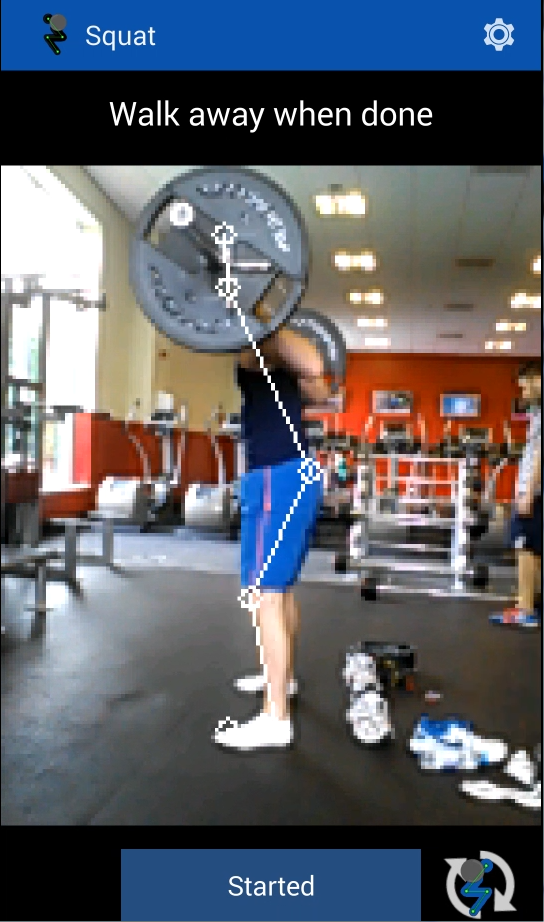
\includegraphics[height=7cm]{evaluation/images/goodbackground1}
    }
    \subfigure{
            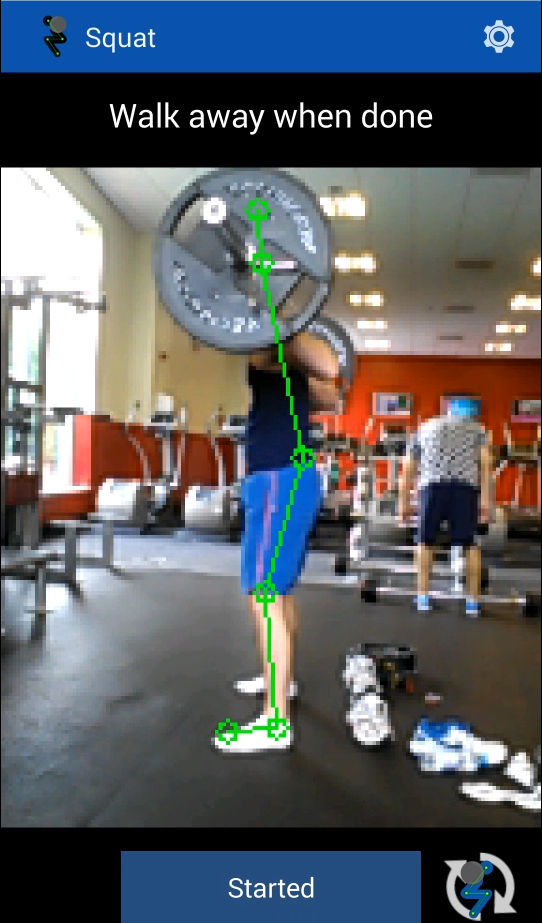
\includegraphics[height=7cm]{evaluation/images/goodbackground2}
    }
    \subfigure{
            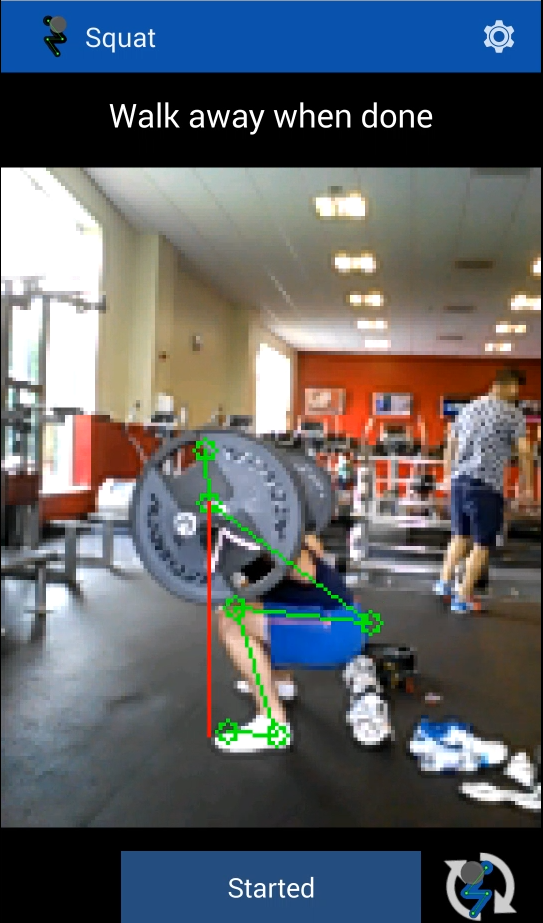
\includegraphics[height=7cm]{evaluation/images/goodbackground3}
    }
\caption{Isolated background movement does not affect tracking}
\label{fig:goodbackground}
\end{figure}

Any movement in the background or foreground that crosses the lifter will effect the subtraction however, as the largest object becomes the combination of the lifter and the disturbance. This can be seen in figure~\ref{fig:badtracking}.

\begin{figure}[H]
    \centering
    \subfigure{
            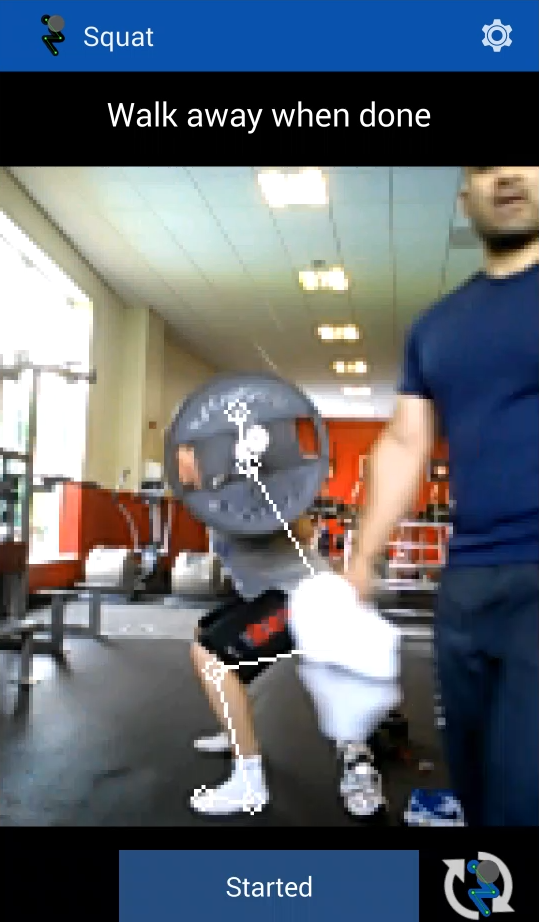
\includegraphics[height=7cm]{evaluation/images/badtracking1}
    }
    \subfigure{
            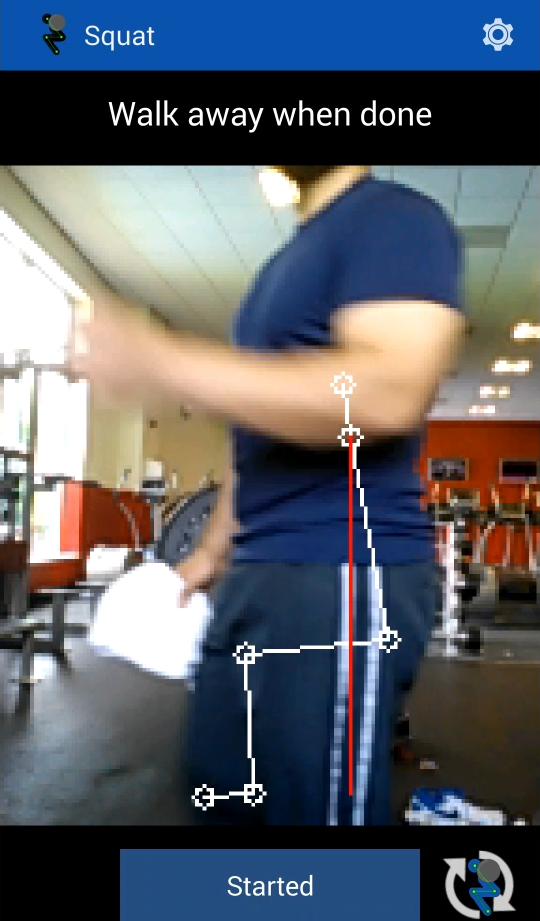
\includegraphics[height=7cm]{evaluation/images/badtracking2}
    }
    \subfigure{
            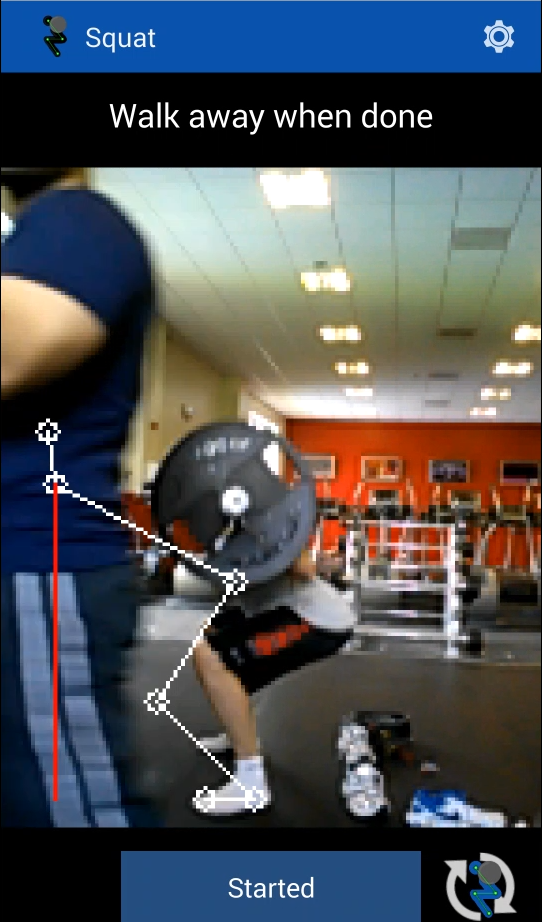
\includegraphics[height=7cm]{evaluation/images/badtracking3}
    }
\caption{A passer by upsets the tracking}
\label{fig:badtracking}
\end{figure}

As the passer-by walks into view, he is detected as foreground, and as soon as he crosses the lifter, becomes part of the largest object, pulling the model towards him. The model follows the passer by until he leaves the view, but after this the model is reasonably quick to snap back into place and continue tracking the lifter as usual.

In unstable lighting conditions, the background subtraction algorithm is prone to failure. When the lighting changes, the colour of pixels in the background will change and (as soon as the difference is greater than the threshold) will be detected as foreground. This then breaks down the tracking - wherever the model resides it achieves maximum overlap with the foreground, and so ceases to move. Perhaps the background subtraction algorithm could be improved to update its known background over time, allowing for variations in lighting. This is discussed further in section~\ref{sec:future_bgsub}.

From the screenshots above, it can be seen that the application tracks reasonably well on the whole. The joint locations of the model do not always perfectly match the lifter, but the model follows the lifter with reasonable precision. The proportions of the model are fixed in the current implementation, which is likely the cause of any intermittent joint misalignment.

The combination of background subtraction, model and optimisation tracks the lifter well overall, and is robust to a reasonable level of movement in the surrounding area.

\subsection{Analysis}
\label{sec:analysis_eval}

As the application analyses squat form using computer vision, it is difficult to evaluate it quantitatively. It is possible however to compare the scores given by the application with scores given by an expert observing the squat, to give a semi-quantitative measure of the application's performance.

In an experiment, 84 squats were performed, observed both by the application and an expert. Figure~\ref{fig:scorediff} shows a radar chart with the expert awarded scores in blue, and the application awarded scores in red:

\begin{figure}[H]
    \centering
	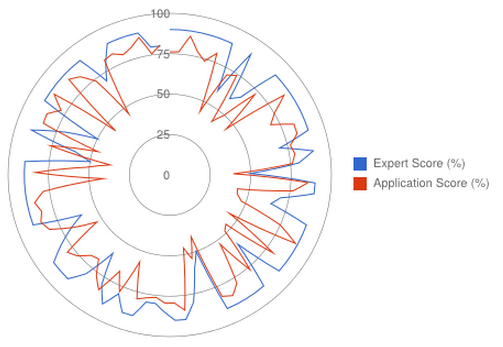
\includegraphics[height=6cm]{evaluation/images/scores_difference}
\caption{Expert awarded scores plotted against application awarded scores}
\label{fig:scorediff}
\end{figure}

Of the 84 squats scored, 17 did not track accurately throughout the lift (likely due to changes in lighting conditions). Removing these repetitions gives the following results in figure~\ref{fig:scorediffgood}.

\begin{figure}[H]
    \centering
	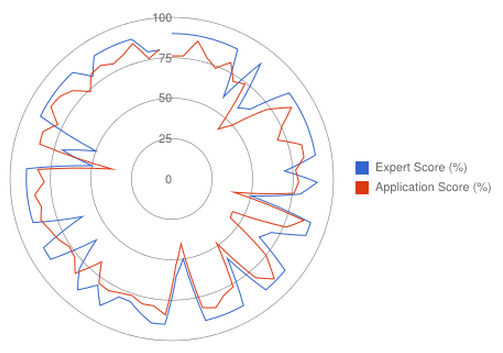
\includegraphics[height=6cm]{evaluation/images/scores_difference_goodtrack}
\caption{Expert awarded scores plotted against application awarded scores, with inaccurately tracked repetitions removed}
\label{fig:scorediffgood}
\end{figure}

The full dataset gathered for this experiment is available in the appendix (section \ref{sec:analysis_eval_scores}).

The figures show the lines following similar paths, meaning that the application scores squats in a similar manner to an expert. With squats that did not track correctly included, the Pearson product-moment correlation coefficient is 0.37, which shows a reasonable positive correlation between the expert awarded scores and the application awarded scores. Removing the incorrectly tracked squats, the correlation coefficient is 0.68, which shows a strong positive correlation, meaning that when an expert scores a squat highly, the application is also likely to score the squat highly.

On average, the expert awarded a score around 7.5\% higher than the application (excluding squats incorrectly tracked). This was largely due to penalties for the angle at the knees expanding at a faster rate than that of the hips, where the difference in rate was near-negligible and could not be spotted by eye.

From these results it can be seen that the application, although less generous, scores squats relative to one another in a similar manner to an expert. Thus it can be concluded that the application offers reasonably accurate analysis of squat form.

\section{Resource Usage}

Another way in which the application can be evaluated is by its use of resources. Resources on a mobile device include the CPU, battery and memory.

\subsection{CPU and Battery Usage}
In terms of CPU usage, this application is quite resource intensive. Processing video frames in real-time means that the CPU is used constantly while the application is running. This level of CPU usage can be expected by a user however, as it is widely understood that video processing (especially that which runs in real-time) requires a large proportion of CPU time.

The amount of CPU usage has a knock-on effect on the power consumption. It was measured that running the tracking stage of the algorithm over a time period of 2 minutes and 56 seconds, the battery level of the Samsung Galaxy S4 was drained by 2\%. This is quite a high consumption rate, although not significantly higher than that of the Samsung Camera application, which drained 2\% of the battery over 4 minutes and 12 seconds. The application is unlikely to be used for long periods of time, and so consumption for this application is less of a concern than it would be for a background service for example. A lifter will on average perform squats for no longer than 30 minutes including rest periods, and so we can estimate that the application will drain the battery of the mobile device by approximately 20\% over the course of a particularly long session, which is not unreasonable.

\subsection{Memory Usage}
Memory usage was monitored during the running of the application using the Android command:

\texttt{adb shell dumpsys meminfo <package\_name>}

This provides an output of the current memory usage of the application. On average, the application used around 63MB of RAM. Of this, 56MB was `private dirty' memory, which details the RAM that is used solely by the application, and cannot be swapped into virtual memory or shared with another application.

We can compare this memory usage to other Android applications. The following table shows the memory usage of this application against other common applications:

\begin{figure}[H]
    \centering
	\begin{tabular}{ | l | c | }
	    \hline
	    \textbf{Application} & \textbf{Average Memory Usage (MB)} \\ \hline
	    Facebook & 109 \\ \hline
	    Squat! & 63 \\ \hline
	    Instagram & 44 \\ \hline
	    YouTube & 41 \\ \hline
	    GMail & 25 \\ \hline
	    Samsung Camera & 25 \\
	    \hline
    \end{tabular}
\caption{Average Memory Usage of Common Android Applications}
\label{fig:memusage}
\end{figure}

As shown in figure~\ref{fig:memusage}, the application's memory usage is greater than most common applications, however it is not outrageously high, being less than that of Facebook - a very widely used application.

It can be concluded that although fairly resource intensive, the application does not use an impractical level of resources and is therefore suitable for use in this regard.

\section{User Testing Evaluation}
\label{sec:user_testing}
In addition to the evaluation against the goal, the application was also evaluated by a set of three users. These users are gym-goers of differing experiences: Harry Stevenson has been lifting weights for around three months, Greg Pye has been training for a little over a year, and Tom Wilding has been lifting for around four years.

These users took the application to the gym installed on a mobile device, and spent time using it to analyse their squat form.

They were asked to answer the following questions with a score out of 10 and a few words to gauge the success of the application:

\begin{enumerate}
    \item Was the application intuitive and easy to use?
    \item Was the application accurate in its tracking and analysis?
    \item Did the application aid in your training?
\end{enumerate}

They were also asked to provide any additional feedback from their real-world use of the application.

\pagebreak
\subsection{Intuitiveness and Ease of Use}

Harry Stevenson:
\begin{quote}
\textbf{9/10} \emph{I felt that the app was very easy to use and the instructions that were given were clear enough so that I could understand it easily. The text-to-speech element helped me understand the instructions even though my phone was on the other side of the room.}
\end{quote}

Greg Pye:
\begin{quote}
\textbf{9/10} \emph{Very easy to use with verbal and text prompts and a simple interface. I think it'll take a user a couple of attempts of using the app with no prior instructions or help in terms of it needing the background to be still and you need to select which way to face. But after one or two tries I think it's a doddle to use.}
\end{quote}

Tom Wilding:
\begin{quote}
\textbf{9/10} \emph{The app is very intuitive because of its simplistic UI and real-time voice feedback. It could highlight more the fact that the camera needs to be completely still and that there must be no one in view at the start.}
\end{quote}

\subsection{Accuracy in Tracking and Analysis}

Harry Stevenson:
\begin{quote}
\textbf{7/10} \emph{The app mostly tracked my body correctly, however on a few occasions the skeleton would track other objects or would move from my body. The analysis of the squat form was very accurate and provided useful feedback for my future use in the gym.}
\end{quote}

Greg Pye:
\begin{quote}
\textbf{9/10} \emph{As long as conditions are good the app recognises and tracks very well. Certainly far higher accuracy than I would ever expect from running such real-time processing on a phone and from its own camera too.}
\end{quote}

Tom Wilding:
\begin{quote}
\textbf{10/10} \emph{The application was capable of tracking accurately and provided relevant tips on depth and form. The tracking is particularly impressive as it just uses the camera with no manual calibration or tracking points.}
\end{quote}

\pagebreak
\subsection{Training Aid}

Harry Stevenson:
\begin{quote}
\textbf{9/10} \emph{The app was very beneficial in my personal training as it showed me where I had been going wrong on my form for the past three months. This app most likely saved me from having some sort of knee injury and so I found it thoroughly useful.}
\end{quote}

Greg Pye:
\begin{quote}
\textbf{7/10} \emph{I have pretty good squat form to begin with. But it did highlight a tendency at times to be a bit further forward than needs be. Nothing major to correct but will definitely keep an eye on that.}
\end{quote}

Tom Wilding:
\begin{quote}
\textbf{8/10} \emph{The application provides good real-time feedback and visualisation however it is difficult to see the screen whilst undertaking the exercise as the camera must be positioned adjacent to the user. For me, the application was mainly helpful as a guide, to check form and depth, however would be impractical to set up every time when training. I think it would be very useful for a beginner to learn independently how to improve technique.}
\end{quote}

\subsection{Additional Feedback}

Harry Stevenson:
\begin{quote}
\emph{Sometimes the text-to-speech element would put off other gym-goers. It was sometimes difficult to find a place to put the phone so that it would stay still enough for proper usage, and in those places it did not quite have the correct angle to cover my whole body.}
\end{quote}

Greg Pye:
\begin{quote}
\emph{I think it's a great app - only limited by a gym being busy and so hard to get a still background, especially during peak times. It would be good if the app could record the session so you could play back. This means you can see how good the tracking actually was to come up with the rep's score and also watch your squat form too. I think that will be useful - especially for someone training on their own.}
\end{quote}

Tom Wilding:
\begin{quote}
\emph{Although a third party screen recording application can be used to record the analysis, it would be good if the application recorded each set for later review. Perhaps a more detailed analysis could be provided or slow motion replays after the real-time analysis.}
\end{quote}

\subsection{Summary of User Evaluation}

From the feedback received, the project can be evaluated as a success, meeting the goal of providing accurate real-time feedback on squat form to aid in training. Whilst not always practical for everyday use at the gym due to the overhead of finding a position to rest the mobile device, it was deemed a very useful tool for beginners to learn correct squat technique without an expert guiding them.